\documentclass{article}
\usepackage[margin=3cm]{geometry}

\usepackage{graphicx}
\usepackage{float}

\begin{document}
	
	\title{
		\line(1,0){500}\\
		[6mm]
		\bfseries Architectural Requirements Specifications and Design 
		\\
		[6mm] 
		NavUP System
		\line(1,0){500}\\
		[15mm]}
	
	\author{
		Josef Alberts - 14395283\\ 
		Gregory Austin - 14039712\\ 
		Jocelyn Bondjobo - 13232852\\ 
		Claudio Da Silva - 14205892\\ 
		Thomas Honiball - 15348751\\
		Lesego Makaleng - 15175716}
	
	\maketitle{}
	\pagebreak
	\tableofcontents
	\pagebreak

		
	\section{Introduction}
	
	The architectural requirements specification and design document, is aimed at identifying the architectural and design aspects of the system, with regards to the NavUP system in this particular instance
	
		\subsection{Purpose}
		
		The purpose of this document will be to determine the best course of action with regards to architectural design, including the requirements set forth, the constraints placed upon it and the design decisions going forward,including the architectural patterns, system design and technologies selected to solve the various requirements and constraints that have been identified.
	
		\subsection{Definitions, Acronyms, and Abbreviations}
			
			\begin{itemize}
				
				\item \textbf{GIS} \textbf{\textit{(Geographic Information System)}} \\
				\newline
				A geographic information system (or GIS) is a system designed to capture, store, manipulate, analyze, manage, and present spatial or geographic data.\\
				
				\item \textbf{GPS} \textbf{\textit{(Global Positioning System)}} \\
				\newline
				A radio navigation system that allows land, sea, and airborne users to determine their exact location, velocity, and time 24 hours a day, in all weather conditions, anywhere in the world.
			
			\end{itemize}

	\section{Requirements and Constraints}
		
		\subsection{External Interface Requirements}
		
			\subsubsection{User interfaces}
			
				\begin{figure}[H]
					
					\centering{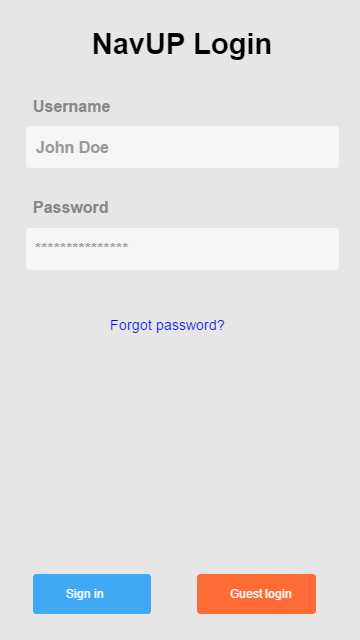
\includegraphics[width=0.25\linewidth]{./images/mocks/login_page.jpg}}
					\caption{Login Page}
					
					
				\end{figure}
			
				With regards to the login page (Figure 1), it is important to note the lack of distraction and the clear and concise labels given to each element. This ensures users of any kind have a simple straight forward means of using the application. Both sign in and guest login are provided as options, as well as a password recovery means.
			
				\begin{figure}[H]
					
					\centering{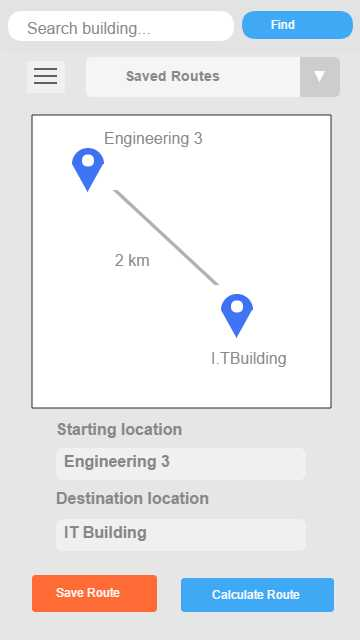
\includegraphics[width=0.25\linewidth]{./images/mocks/main_page.jpg}}
					\caption{Main Page}
				
				\end{figure}

				With regards to the main page (Figure 2), we see that all the options are presented in an easy to understand way. Elements which take up minimal room yet offer a lot such as drop-down boxes are used in order to save space and look neat, but provide the user with all the requirements in plain sight. We see a method to both calculate and select routes is available, as well as a method to search for what is required. The most important thing to note is the map being the center of attention, as it is the most important part of the application, it is made to stand out and take the focus of the user.
			
				\begin{figure}[H]
					
					\centering{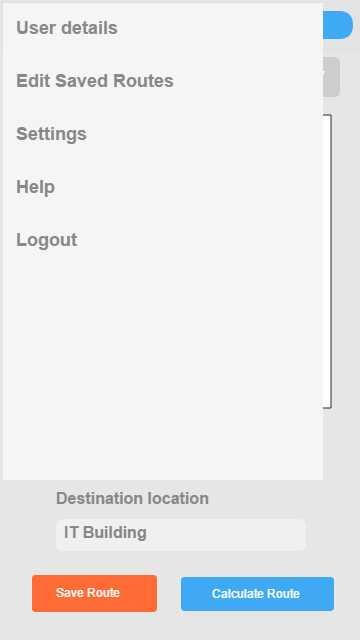
\includegraphics[width=0.25\linewidth]{./images/mocks/navigation_page.jpg}}
					\caption{Navigation Bar On Main Page}
					
				\end{figure}
			
				With regards to the navigation bar (Figure 3), we see that it is called via the hamburger button present on the main page(Figure 2) and the user page (Figure 4). This ensures that navigation is available wherever needed. Most importantly though, it ensures that the help item provided is always available when anybody is stuck, as well as the option to logout whenever needed. By keeping a consistent navigation menu, we also ensure that all pages will be the same, thus users will not be required to search hours for a button that might be in a different location or not exist on that page.
			
				\begin{figure}[H]
					
					\centering{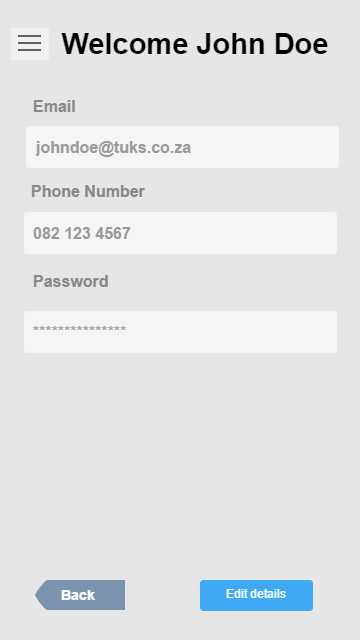
\includegraphics[width=0.25\linewidth]{./images/mocks/user_page.jpg}}
					\caption{User Details Page}
					
				\end{figure}
			
				With regards to the user details page(Figure 4), we see that a concise and easy display with clear labels is given to allow users to change the details they need, while keeping important identification factors like Usernames the same, and not giving the option to change them. We see again navigation is present, as well as an easy method of returning to the main screen. \\
				
				With regards to all the figures, a constant font and colour should be used throughout, and should preferably make accommodation for various disabilities such as colour blindness, thus not being too colorful, or visual impairment, thus not making text too small. The layout should remain consistent across resolutions and should accommodate as many different models of device as possible, from phone to tablet and more.\\
				
				While not explicitly shown, a preferably non-mobile administrator management page should be given to allow those running the server side of the system to make changes. This page would be required to be intuitive, but not necessarily appealing.
			
			\pagebreak
			
			\subsubsection{Hardware interfaces}
			
			The device types used by the system are thought to be mobile devices such as phones and tablets, as well as a physical computer on which to run the server itself.\\
			
			The system makes use of the internal hardware of the device it is on, interacting with things such as:
			
				\begin{itemize}
					\item The device's GPS, via internal means, thus natively connecting via the device's operating system in order to collect location data.
					\item The device's Internet connection, via internal means, thus natively connecting via the device's operating system in order to pull outside data.
				\end{itemize}
			
			The system however also plans to make use of some external devices, such as:
			
				\begin{itemize}
					\item Cameras, placed around the campus in order to deal with traffic detection and possibly provide heat-maps, it would communicate to the server via the internal network and the server with the device via JSON calls .
				\end{itemize}
			
			\subsubsection{Software interfaces}
			
			As stated, the system will consist of two main components, the Server and the Client.The Server is to be run off a high powered computing device, and the client side shall be run off a mobile device such as a phone or tablet. The communication method between these two modules will be that of a REST API. This means that the two components will communicate via an Internet connection, where JSON data is sent between the two components in order to transfer the required data.\\
			
			The server will connect with a database in order to store information, likely via a native connection built into the server architecture.\\
			
			The client will communicate with the internal structure of the device via native libraries, such as Android's native GPS API.
			
			\subsubsection{Communication interfaces}
			
			The software is to make use of the following communication protocols:
			
				\begin{itemize}
					\item REST, which will be the foundation of delivering data between the server and the client.
					\item Native Notifications, to allow a device to deliver information from inside the application to the recipient.
					\item Email protocols such as SMTP, to allow sending of emails for things such as verification or other updates.
					\item SMS protocols, as stated in the requirements SMS may be implemented as a notification method, and thus require an SMS server to broadcast.
				\end{itemize}
		
		\pagebreak
		
		\subsection{Design Constraints}
		
		\subsection{Software System Attributes}
	
	\pagebreak
	
	\section{Module Design}
	
		\subsection{GIS Subsystem}

		\subsection{Notification Subsystem}
	
		\subsection{Navigation Subsystem}
	
		\subsection{Events Subsystem}
	
	\pagebreak
	
	\section{System assessment}	
	
		\subsection{Technology choices}
	
		\subsection{Quality and Feasibility of Design}
	

\end{document}
